\swjtuChapter{系统详细设计报告}

% 去掉章节前缀，使用 1 / 1.1 / 1.1.1 的编号体系
\setcounter{section}{0}
\renewcommand{\thesection}{\arabic{section}}
\renewcommand{\thesubsection}{\thesection.\arabic{subsection}}
\renewcommand{\thesubsubsection}{\thesubsection.\arabic{subsubsection}}

\section{引言}

\subsection{编写目的}
本文档在《软件需求规格说明书》和《系统概要设计报告》的基础上，对系统核心模块进行部件级细化设计，明确前后端交互、类与接口职责、关键业务时序及异常处理策略，为编码实现、联调测试和后期运维提供统一依据。

\subsection{项目背景}
“零售物品智能识别系统”面向商超场景，目标是打通顾客侧“搜索/识别/下单”链路与管理侧“商品维护/库存预警/摄像头巡检”链路。当前项目由四个子系统组成：
\begin{itemize}[leftmargin=2em]
  \item \textbf{retail-admin-pro}：管理端前端（Vue3 + Vite）。
  \item \textbf{retail-customer}：微信小程序客户端。
  \item \textbf{retail-server}：Spring Boot 后端服务，负责业务编排与数据一致性。
  \item \textbf{retail-ai}：FastAPI AI 服务，提供摄像头、识别、搜索能力。
\end{itemize}

\subsection{参考文献}
\begin{enumerate}[leftmargin=2em]
  \item 《软件工程：实践者的研究方法》
  \item Spring Boot 3.3 官方文档
  \item FastAPI 官方文档
  \item 微信小程序开发文档
  \item MyBatis-Plus 官方文档
\end{enumerate}

\section{系统功能需求概要}

系统按业务闭环划分为三个主模块：
\begin{enumerate}[leftmargin=2em]
  \item \textbf{智能视觉导购模块}：支持文本检索、图片识别、货架定位。
  \item \textbf{交易与结算模块}：支持购物车管理、库存校验、订单生成、支付确认。
  \item \textbf{后台商品与库存监控模块}：支持商品维护、摄像头管理、告警处理、定时巡检。
\end{enumerate}

模块间关系如下：
\begin{itemize}[leftmargin=2em]
  \item 顾客侧通过小程序与后端交互，后端按需转发 AI 能力调用。
  \item 管理员侧通过管理端维护主数据与调度参数。
  \item 交易成功后触发库存与告警联动，低库存时由后台机制继续触发补给流程。
\end{itemize}

\begin{center}
  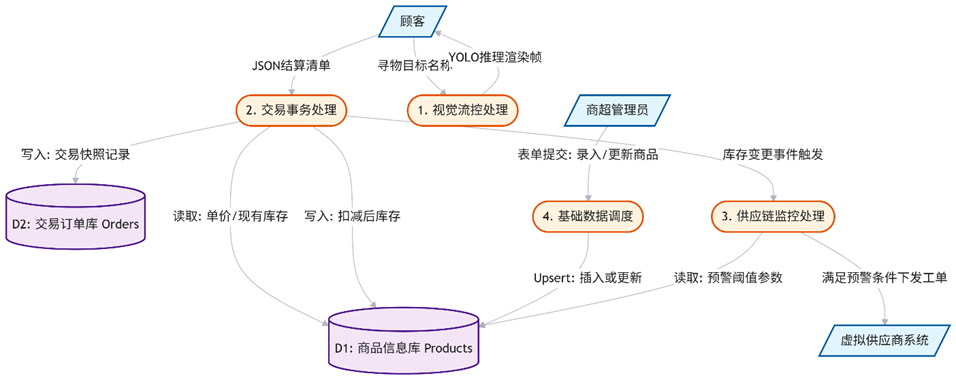
\includegraphics[width=0.9\textwidth]{images/图3-9.png}\\[0.3em]
  {\zihao{-5}图3-1\quad 系统一层数据流（用于功能分解映射）}
\end{center}

\section{智能视觉导购模块详细设计}

\subsection{功能模块概述}
智能视觉导购模块聚焦"找得到、看得见、加得进购物车"，主要功能为：
\begin{itemize}[leftmargin=2em]
  \item 文本检索：小程序调用 \texttt{GET /api/goods/page} 通过名称模糊搜索与分类筛选查找商品。
  \item 图片识别：小程序上传 base64 图像至 \texttt{POST /api/applet/scan}，后端调用 \texttt{POST /api/ai/recognize/center} 返回去重后的 Top-K 商品候选。识别请求具备重试机制——后端最多重试 2 次（间隔 1s/2s），前端也支持最多 2 次自动重试，保障网络波动下的可用性。
  \item 商品详情补全：通过 \texttt{POST /api/applet/goods/listByIds} 将识别出的 ID 列表转换为可展示的商品信息。
\end{itemize}

\subsection{用户交互界面设计}
顾客端对应页面与交互如下：
\begin{enumerate}[leftmargin=2em]
  \item \textbf{查询页（pages/search）}：输入关键词，实时节流检索，展示结果与推荐流。点击"加入购物车"按钮直接添加 1 件商品到购物车（无需二次确认），展开 +/- 数量控件后增减操作自动同步购物车，数量减至 0 时自动移出购物车。
  \item \textbf{识别页（pages/scan）}：拍照或相册选图后，发起识别并在页面展示去重后的候选商品。识别接口支持前后端双重重试机制，确保弱网环境下的成功率。识别结果按商品类别去重，避免同一商品重复展示。
  \item \textbf{商品详情页（pages/goods）}：查看单品信息并加入购物车。
\end{enumerate}

交互设计原则：
\begin{itemize}[leftmargin=2em]
  \item 请求期间给出加载态，避免重复点击。
  \item 识别失败自动重试，最终失败时提示友好错误信息。
  \item 商品加入购物车后即时反馈，并更新购物车角标；加减购操作直接同步后端，无需额外确认步骤。
\end{itemize}

\subsection{类及接口细化设计}

\subsubsection{核心类与职责}
\begin{itemize}[leftmargin=2em]
  \item \texttt{AppletCameraController}：接收 \texttt{image\_base64}，调用 AI 聚合服务。
  \item \texttt{AppletGoodsController}：按 ID 批量查询商品详情。
  \item \texttt{GoodsController}：提供商品分页检索（按名称模糊搜索 + 分类筛选 + 价格排序）。
  \item \texttt{AiIntegrationServiceImpl}：统一封装与 Python AI 的 HTTP 调用，内置去重逻辑与最多 2 次自动重试。
  \item \texttt{recognition/routes.py}：实现中心点识别（按类别去重）与批量货架识别。
\end{itemize}

\subsubsection{关键接口说明}
\begin{center}
  \renewcommand{\arraystretch}{1.35}
  \zihao{5}
  \begin{tabular}{|>{\centering\arraybackslash}m{3.6cm}|>{\centering\arraybackslash}m{2.2cm}|>{\centering\arraybackslash}m{6.4cm}|}
    \hline
    \textbf{接口} & \textbf{方法} & \textbf{说明} \\ \hline
    /api/goods/page & GET & 商品分页检索，参数 \texttt{name}、\texttt{categoryId}、\texttt{page}、\texttt{size} \\ \hline
    /api/applet/scan & POST & 图片识别，参数 \texttt{image\_base64}、\texttt{k} \\ \hline
    /api/applet/goods/listByIds & POST & 按商品 ID 列表批量查询详情 \\ \hline
    /api/ai/recognize/center & POST & AI 中心点识别（内部接口，已去重） \\ \hline
  \end{tabular}
  \\[0.3em]
  {\zihao{-5}表3-1\quad 视觉导购模块关键接口}
\end{center}

\subsubsection{时序细化（文字时序）}
识别寻物主流程的时序如下：
\begin{enumerate}[leftmargin=2em]
  \item 顾客在小程序选择图片并提交。
  \item 小程序调用 \texttt{POST /api/applet/scan}，前端内置最多 2 次失败自动重试。
  \item 后端调用 AI 服务 \texttt{POST /api/ai/recognize/center} 获取候选 ID（Python 侧已按类别去重），后端内置最多 2 次重试。
  \item Python YOLO 检测器返回距画面中心最近的 k 个不同类别商品的坐标与置信度。
  \item 后端在结果组装阶段执行冗余去重校验，确保无重复商品。
  \item 后端查询商品主数据并补全名称、价格、库存、货架号。
  \item 后端返回候选列表；前端展示并支持加减购操作。
\end{enumerate}

\section{交易与结算模块详细设计}

\subsection{功能模块概述}
交易与结算模块负责购物车数据管理、订单结算、库存扣减及订单查询。关键约束为“库存扣减与订单写入必须同事务提交，失败则整体回滚”。

\subsection{用户交互界面设计}
顾客端交互主要在以下页面完成：
\begin{itemize}[leftmargin=2em]
  \item \textbf{购物车页（pages/cart）}：增减数量、勾选商品、清空购物车、进入结算。
  \item \textbf{订单页（pages/order）}：确认结算、查看历史订单、按状态筛选。
  \item \textbf{支付页（pages/payment）}：余额/微信支付方式选择与支付确认。
\end{itemize}

界面状态设计：
\begin{enumerate}[leftmargin=2em]
  \item 购物车为空时禁止结算。
  \item 结算中使用按钮锁定和 Loading，防止重复提交。
  \item 支付成功后跳转用户中心并刷新订单状态。
\end{enumerate}

\subsection{类及接口细化设计}

\subsubsection{核心类与职责}
\begin{itemize}[leftmargin=2em]
  \item \texttt{CartController} + \texttt{CartServiceImpl}：维护 Redis 购物车。
  \item \texttt{OrderController} + \texttt{OrderServiceImpl}：执行结算事务与订单查询。
  \item \texttt{GoodsMapper}：提供 \texttt{selectByIdForUpdate} 与 \texttt{decreaseStock} 原子扣减能力。
  \item \texttt{OrderItemMapper}、\texttt{InventoryLogMapper}：写入明细与库存流水。
\end{itemize}

\subsubsection{结算流程关键逻辑}
\begin{enumerate}[leftmargin=2em]
  \item 从 Redis 读取用户购物车并校验合法性。
  \item 对商品 ID 排序后逐条加锁（\texttt{FOR UPDATE}）降低并发死锁概率。
  \item 校验库存并执行条件扣减（\texttt{stock >= quantity}）。
  \item 写入库存日志，低于阈值时生成库存告警。
  \item 写入订单主表与订单明细表。
  \item 事务提交后异步清空 Redis 购物车。
\end{enumerate}

\subsubsection{关键接口说明}
\begin{center}
  \renewcommand{\arraystretch}{1.35}
  \zihao{5}
  \begin{tabular}{|>{\centering\arraybackslash}m{3.6cm}|>{\centering\arraybackslash}m{2.2cm}|>{\centering\arraybackslash}m{6.4cm}|}
    \hline
    \textbf{接口} & \textbf{方法} & \textbf{说明} \\ \hline
    /api/cart/add & POST & 加入/修改购物车商品数量 \\ \hline
    /api/cart/list & GET & 查询当前用户购物车 \\ \hline
    /api/order/checkout & POST & 管理端/通用结算接口 \\ \hline
    /api/applet/order/checkout & POST & 小程序结算接口（可携带清单） \\ \hline
    /api/applet/order/pay & POST & 小程序订单支付确认 \\ \hline
    /api/order/list & GET & 查询订单历史 \\ \hline
  \end{tabular}
  \\[0.3em]
  {\zihao{-5}表3-2\quad 交易与结算模块关键接口}
\end{center}

\section{后台商品与库存监控模块详细设计}

\subsection{功能模块概述}
该模块面向管理员与系统后台任务，完成商品全生命周期管理、库存告警治理、摄像头绑定与巡检调度。核心能力包括：
\begin{itemize}[leftmargin=2em]
  \item 商品分页查询、新增、编辑、删除、图片上传。
  \item 告警分页查询、告警处理、未处理告警聚合。
  \item 摄像头绑定、预览、流式代理、调度参数动态更新。
  \item 定时巡检调用 AI 批量识别并同步货架商品信息。
\end{itemize}

\subsection{用户交互界面设计}
管理端对应页面如下：
\begin{enumerate}[leftmargin=2em]
  \item \textbf{商品管理页（views/goods/manage）}：搜索、增删改、库存可视标签、图片上传。
  \item \textbf{视觉调度页（views/camera/schedule）}：摄像头绑定、预览、巡检配置、手动触发。
  \item \textbf{数据看板页（views/dashboard/dataVisualize）}：展示销售、库存和告警概览。
\end{enumerate}

\subsection{类及接口细化设计}

\subsubsection{核心类与职责}
\begin{itemize}[leftmargin=2em]
  \item \texttt{GoodsController}：商品 CRUD 与库存补货日志触发。
  \item \texttt{WarningController} / \texttt{AdminWarningController}：告警分页与待处理清单。
  \item \texttt{CameraController}：摄像头管理与流代理接口。
  \item \texttt{CameraScanScheduler}：定时任务调度、分批调用 AI、同步货架信息。
  \item \texttt{GlobalExceptionHandler}：统一异常转换与错误码输出。
\end{itemize}

\subsubsection{调度时序细化（文字时序）}
\begin{enumerate}[leftmargin=2em]
  \item 定时器按 \texttt{interval-minutes} 触发巡检任务。
  \item 读取状态正常的摄像头列表并按 \texttt{batch-size} 分批。
  \item 后端向 \texttt{/api/ai/recognize/shelf/batch} 提交批量识别请求。
  \item 收到 \texttt{detected\_goods\_ids} 后回写商品 \texttt{shelf\_id}。
  \item 输出巡检日志，供管理员在页面和日志系统中查看。
\end{enumerate}

\subsubsection{关键接口说明}
\begin{center}
  \renewcommand{\arraystretch}{1.35}
  \zihao{5}
  \begin{tabular}{|>{\centering\arraybackslash}m{3.6cm}|>{\centering\arraybackslash}m{2.2cm}|>{\centering\arraybackslash}m{6.4cm}|}
    \hline
    \textbf{接口} & \textbf{方法} & \textbf{说明} \\ \hline
    /api/goods/page & GET & 商品分页查询 \\ \hline
    /api/goods & POST/PUT & 商品新增与编辑 \\ \hline
    /api/warning/page & GET & 告警分页查询 \\ \hline
    /api/warning/\{id\}/resolve & PUT & 告警处理 \\ \hline
    /api/admin/camera/list & GET & 摄像头列表 \\ \hline
    /api/admin/camera/scheduler/config & GET/PUT & 巡检参数查询与更新 \\ \hline
    /api/admin/camera/scheduler/trigger & POST & 手动触发巡检 \\ \hline
  \end{tabular}
  \\[0.3em]
  {\zihao{-5}表3-3\quad 后台监控模块关键接口}
\end{center}

本章从模块职责、界面交互、类与接口、关键时序四个层面完成了详细设计，后续测试用例与部署方案均以本章为实现依据。
